\documentclass[11pt,a4paper]{article}

% Paquetes esenciales para español, tablas y gráficos
\usepackage[utf8]{inputenc}
\usepackage[T1]{fontenc}
\usepackage[spanish,es-tabla]{babel}
\usepackage{geometry}
\geometry{margin=2.5cm}
\usepackage{booktabs}
\usepackage{graphicx}
\usepackage{array}
\usepackage{multirow}
\usepackage{float}
\usepackage{hyperref}
\usepackage{xcolor}
\usepackage{amsmath}
\usepackage{caption}

\hypersetup{
    colorlinks=true,
    linkcolor=blue!70!black,
    urlcolor=blue!70!black,
    citecolor=blue!70!black
}

\title{\textbf{Evaluación Experimental de Sistemas de Archivos, Almacenamiento y Acceso Remoto Distribuido}\\
\large Contenedor / Estación de Trabajo $\leftrightarrow$ Nodo Edge (Raspberry Pi)}
\author{Sistemas Operativos — Evaluación de Sistemas Distribuidos}
\date{\today}

\begin{document}

\maketitle

\begin{abstract}
Este documento presenta el diseño, implementación y evaluación experimental de un servicio distribuido de almacenamiento e I/O desplegado entre un nodo coordinador/cliente (PC / Contenedor) y un nodo de recursos restringidos (Raspberry Pi). Reutilizando la infraestructura de comunicación de tramas TCP y tolerancia a fallos previamente desarrollada, se acotó el alcance hacia la caracterización rigurosa a nivel de Sistema Operativo de dos formatos de almacenamiento (\textbf{CSV vs. Parquet}), cuatro patrones de acceso (\texttt{read\_full}, \texttt{read\_columns}, \texttt{read\_range} y \texttt{write\_file}), comparación de acceso \textbf{Local vs. Remoto}, dos protocolos de transporte (\textbf{Sockets TCP vs. gRPC}), escalabilidad bajo \textbf{clientes concurrentes} (1 a 8 hilos) y recuperación ante \textbf{fallos del servicio} (\textit{No retry} vs. \textit{Timeout + retry}).
\end{abstract}

\section{Problema, Objetivo y Pregunta de Investigación}

\subsection{Problema y Reducción de Alcance}
Los sistemas distribuidos con nodos de recursos limitados (como una Raspberry Pi) deben gestionar eficientemente el almacenamiento en disco, las operaciones de entrada/salida (I/O) y la transferencia remota de datos. Siguiendo los lineamientos de alcance reducido del proyecto, se prescindió de la sobrecarga de entrenamiento neuronal federado (\textit{FedAvg}) y del tercer nodo, concentrando el banco de pruebas (\textit{testbed}) en la interacción directa y medible entre \textbf{dos nodos}:
\begin{enumerate}
    \item \textbf{Nodo Coordinador y Cliente de Pruebas (PC / Contenedor)}: Ejecuta las pruebas locales de referencia (\textit{Local Baseline}), agenda las baterías de experimentos repetibles y recolecta métricas de latencia ($p_{50}$, $p_{95}$), \textit{throughput} y consumo de recursos.
    \item \textbf{Nodo de Servicio de Archivos e I/O (Raspberry Pi)}: Almacena los conjuntos de datos en formatos CSV y Parquet, procesa lecturas completas, filtradas por columnas, por rangos de filas y escrituras en disco, y monitorea en tiempo real el uso de CPU, memoria RAM y actividad de disco mediante \texttt{psutil}.
\end{enumerate}

\subsection{Pregunta de Investigación}
\begin{quote}
\textit{¿Cómo afectan los formatos de almacenamiento (CSV vs. Parquet), los patrones de acceso y los métodos de transferencia (TCP vs. gRPC) al rendimiento de I/O, el uso de recursos del sistema operativo y la disponibilidad entre un contenedor/PC y una Raspberry Pi?}
\end{quote}

\section{Arquitectura del Sistema e Implementación}

El sistema se estructuró en cuatro módulos principales en Python (\texttt{3.13.15}, \texttt{pandas 3.1.1}, \texttt{pyarrow 26.0.1}, \texttt{grpcio 1.85.1}, \texttt{psutil 7.2.2}):
\begin{itemize}
    \item \textbf{\texttt{prepare\_datasets.py}}: Generador determinístico con semilla fija (\texttt{seed = 42}) basado en el dataset de Calidad del Aire (\texttt{global\_test.csv}). Produce tres tamaños fijos (\texttt{small}, \texttt{medium} y \texttt{large}) en formato CSV y Parquet (compresión \textit{Snappy}), verificando automáticamente la equivalencia lógica (\texttt{np.allclose}) entre ambos formatos.
    \item \textbf{\texttt{server/file\_server.py}}: Servicio de archivos en la Raspberry Pi que expone simultáneamente un servidor de \textbf{Sockets TCP} (puerto \texttt{5000}, con delimitación de tramas de 4 bytes Big-Endian heredada de \texttt{protocol.py}) y un servidor \textbf{gRPC HTTP/2} (puerto \texttt{50051}). Mide aisladamente el tiempo puro de disco (\texttt{server\_disk\_io\_ms}) para separarlo de la sobrecarga de red.
    \item \textbf{\texttt{client/file\_client.py}}: Cliente de evaluación que ejecuta el \textit{baseline} local y las peticiones remotas, desglosando el tiempo total de respuesta (\textit{wall time}) en:
    \[
        T_{\text{total}} = T_{\text{disco I/O}} + T_{\text{serialización}} + T_{\text{red}}
    \]
    \item \textbf{\texttt{run\_storage\_experiments.py}}: Orquestador automatizado que ejecuta los cinco escenarios experimentales (A--E), calcula estadísticos robustos ($p_{50}$, $p_{95}$, desviación estándar $\sigma$) y exporta las evidencias en \texttt{results/per\_run\_metrics.csv} y \texttt{results/summary\_metrics.csv}.
\end{itemize}

\section{Preparación de Datos y Eficiencia de Almacenamiento}

El Cuadro~\ref{tab:datasets} resume las características físicas de los datasets generados con semilla fija (\texttt{seed=42}). Se comprobó que Parquet reduce el espacio en disco entre \textbf{3.12$\times$} y \textbf{7.66$\times$} manteniendo exactamente la misma información lógica de 14 columnas.

\begin{table}[H]
\centering
\caption{Comparación de almacenamiento en disco y razón de compresión (CSV vs. Parquet).}
\label{tab:datasets}
\begin{tabular}{lrrrrcc}
\toprule
\textbf{Dataset} & \textbf{Filas} & \textbf{Columnas} & \textbf{CSV (KB)} & \textbf{Parquet (KB)} & \textbf{Compresión} & \textbf{Equivalencia} \\
\midrule
\texttt{small}  & 1,000  & 14 & 274.24  & 87.79  & $3.12\times$ & Verificada \\
\texttt{medium} & 5,000  & 14 & 1,375.37 & 265.45 & $5.18\times$ & Verificada \\
\texttt{large}  & 20,000 & 14 & 5,515.65 & 720.26 & $7.66\times$ & Verificada \\
\bottomrule
\end{tabular}
\end{table}

\section{Resultados Experimentales}

\subsection{Escenario A: Tamaño de Archivo, Formato (CSV vs. Parquet) y Patrones de Acceso}
Se evaluaron cuatro patrones de acceso: lectura completa (\texttt{read\_full}), proyección de tres columnas (\texttt{read\_columns}: \texttt{['CO(GT)', 'T', 'RH']}), lectura por rango de registros (\texttt{read\_range}: filas 100 a 600) y escritura en disco (\texttt{write\_file}). El Cuadro~\ref{tab:scenario_a} muestra los resultados obtenidos.

\begin{table}[H]
\centering
\caption{Escenario A — Comparación de formatos CSV vs. Parquet según patrón de acceso y tamaño.}
\label{tab:scenario_a}
\resizebox{\textwidth}{!}{%
\begin{tabular}{llrrrrrr}
\toprule
\textbf{Operación} & \textbf{Tamaño} & \textbf{Formato} & \textbf{Latencia $p_{50}$ (ms)} & \textbf{Latencia $p_{95}$ (ms)} & \textbf{Disco I/O (ms)} & \textbf{Serialización (ms)} & \textbf{Red (ms)} \\
\midrule
\multirow{2}{*}{\texttt{read\_full}} & \texttt{large} & CSV & 592.61 & 605.26 & 25.75 & 265.66 & 297.77 \\
 & \texttt{large} & Parquet & \textbf{563.84} & \textbf{583.94} & \textbf{8.47} & 243.79 & 309.54 \\
\midrule
\multirow{2}{*}{\texttt{read\_columns}} & \texttt{large} & CSV & 170.27 & 181.37 & 31.41 & 56.13 & 82.70 \\
 & \texttt{large} & Parquet & \textbf{142.77} & \textbf{166.65} & \textbf{4.65} & 53.67 & 84.74 \\
\midrule
\multirow{2}{*}{\texttt{read\_range}} & \texttt{large} & CSV & \textbf{24.02} & \textbf{42.33} & \textbf{4.39} & 8.01 & 11.36 \\
 & \texttt{large} & Parquet & 25.71 & 45.78 & 8.19 & 7.40 & 10.20 \\
\midrule
\multirow{2}{*}{\texttt{write\_file}} & \texttt{large} & CSV & 556.48 & 577.00 & 536.71 & 0.06 & 19.69 \\
 & \texttt{large} & Parquet & \textbf{55.57} & \textbf{59.12} & \textbf{42.33} & 0.06 & 10.99 \\
\bottomrule
\end{tabular}%
}
\end{table}

\textbf{Interpretación del Escenario A:}
\begin{itemize}
    \item En \textbf{lectura de columnas seleccionadas} (\texttt{read\_columns}), el almacenamiento columnar de Parquet reduce el tiempo puro de lectura en disco de \textbf{31.41 ms a 4.65 ms} ($6.75\times$ más rápido en disco), ya que evita escanear las 11 columnas restantes.
    \item En \textbf{escritura en disco} (\texttt{write\_file}, 20,000 filas), Parquet completa la operación en \textbf{42.33 ms} frente a \textbf{536.71 ms} de CSV ($12.68\times$ más rápido), debido al menor volumen de bytes escritos en bloque binario comprimido frente al formateo de texto línea por línea.
    \item En \textbf{lectura de rangos pequeños al inicio del archivo} (\texttt{read\_range}, filas 100--600), CSV logra un tiempo de disco ligeramente menor (4.39 ms vs. 8.19 ms) porque \texttt{skiprows + nrows} detiene la lectura secuencial inmediatamente sin cargar el grupo de filas (\textit{row group}) completo de Parquet.
\end{itemize}

\subsection{Escenario B: Acceso Local (Baseline) vs. Remoto}
El Cuadro~\ref{tab:scenario_b} contrasta el rendimiento de lectura completa local en la estación de trabajo frente a la petición remota hacia el servicio de archivos.

\begin{table}[H]
\centering
\caption{Escenario B — Desglose de tiempos entre operación Local (Baseline) y Remota.}
\label{tab:scenario_b}
\begin{tabular}{lllrrrrr}
\toprule
\textbf{Tamaño} & \textbf{Formato} & \textbf{Modo} & \textbf{$p_{50}$ (ms)} & \textbf{$p_{95}$ (ms)} & \textbf{Disco I/O (ms)} & \textbf{Serialización (ms)} & \textbf{Red (ms)} \\
\midrule
\multirow{2}{*}{\texttt{small}} & Parquet & Local & 12.79 & 14.59 & 5.88 & 5.77 & 0.00 \\
 & Parquet & Remoto & 35.49 & 38.00 & 5.55 & 13.95 & 15.79 \\
\midrule
\multirow{2}{*}{\texttt{medium}} & Parquet & Local & 30.18 & 39.36 & 6.73 & 22.45 & 0.00 \\
 & Parquet & Remoto & 151.58 & 155.73 & 6.14 & 65.54 & 76.66 \\
\midrule
\multirow{2}{*}{\texttt{large}} & Parquet & Local & 96.91 & 97.51 & 9.86 & 82.13 & 0.00 \\
 & Parquet & Remoto & 560.99 & 573.09 & 7.88 & 251.08 & 305.14 \\
\bottomrule
\end{tabular}
\end{table}

\textbf{Interpretación del Escenario B:} Se demuestra experimentalmente que el tiempo de acceso a disco (\texttt{Disco I/O}) permanece prácticamente constante entre el modo local y remoto ($\approx 7.88$--$9.86$~ms para 20,000 filas en Parquet), mientras que en el acceso remoto el \textbf{98.6\% de la latencia total} corresponde a la serialización/deserialización de estructuras y la transmisión por red.

\subsection{Escenario C: Transporte por Sockets TCP vs. gRPC}
El Cuadro~\ref{tab:scenario_c} compara la transferencia del mismo conjunto de datos lógico utilizando el protocolo de tramas sobre Sockets TCP (\texttt{protocol.py}) frente a llamadas remotas de procedimiento con \textbf{gRPC}.

\begin{table}[H]
\centering
\caption{Escenario C — Comparación de transporte TCP Sockets vs. gRPC (\texttt{read\_full}).}
\label{tab:scenario_c}
\begin{tabular}{lllrrrrr}
\toprule
\textbf{Tamaño} & \textbf{Formato} & \textbf{Transporte} & \textbf{$p_{50}$ (ms)} & \textbf{$p_{95}$ (ms)} & \textbf{Disco I/O (ms)} & \textbf{Red (ms)} & \textbf{Throughput (MB/s)} \\
\midrule
\multirow{2}{*}{\texttt{small}} & CSV & TCP & 60.27 & 74.96 & 4.80 & 41.99 & 4.71 \\
 & CSV & gRPC & \textbf{34.43} & \textbf{44.34} & 4.31 & \textbf{16.84} & \textbf{8.24} \\
\midrule
\multirow{2}{*}{\texttt{medium}} & Parquet & TCP & 164.25 & 182.30 & 6.45 & 92.87 & 8.65 \\
 & Parquet & gRPC & \textbf{154.13} & \textbf{161.97} & 5.84 & \textbf{80.96} & \textbf{9.21} \\
\midrule
\multirow{2}{*}{\texttt{large}} & Parquet & TCP & \textbf{541.74} & \textbf{558.12} & 9.02 & \textbf{280.64} & \textbf{10.51} \\
 & Parquet & gRPC & 551.83 & 593.21 & 8.78 & 292.16 & 10.32 \\
\bottomrule
\end{tabular}
\end{table}

\textbf{Interpretación del Escenario C:} Para cargas pequeñas y medianas (\texttt{small} y \texttt{medium}), \textbf{gRPC} ofrece menor latencia $p_{50}$ y $p_{95}$ que la apertura de sockets TCP individuales por petición. En cargas grandes (\texttt{large}, $\approx 5.8$~MB transmitidos), el encuadre ligero de 4 bytes sobre TCP alcanza un \textit{throughput} ligeramente superior ($10.51$~MB/s vs. $10.32$~MB/s) con menor consumo de CPU en el servidor.

\subsection{Escenario D: Escalabilidad con Clientes Concurrentes}
Se incrementó el número de hilos clientes simultáneos ($C \in \{1, 2, 4, 8\}$) realizando peticiones concurrentes de lectura sobre el dataset \texttt{medium} (5,000 filas).

\begin{table}[H]
\centering
\caption{Escenario D — Impacto de la concurrencia en latencia, Disco I/O y memoria RAM.}
\label{tab:scenario_d}
\begin{tabular}{rlrrrrrr}
\toprule
\textbf{Clientes ($C$)} & \textbf{Formato} & \textbf{$p_{50}$ (ms)} & \textbf{$p_{95}$ (ms)} & \textbf{$\sigma$ (ms)} & \textbf{Disco I/O (ms)} & \textbf{Throughput (MB/s)} & \textbf{RAM Pico (MB)} \\
\midrule
1 & Parquet & 140.95 & 152.51 & 12.84 & 5.34 & 10.16 & 192.39 \\
2 & Parquet & 289.85 & 304.60 & 62.70 & 6.33 & 4.90 & 192.93 \\
4 & Parquet & 489.03 & 590.67 & 81.59 & 126.69 & 2.94 & 200.21 \\
8 & Parquet & 893.88 & 1301.06 & 311.01 & 254.08 & 1.59 & 205.25 \\
\midrule
1 & CSV & 133.40 & 142.15 & 9.72 & 11.60 & 10.70 & 191.98 \\
2 & CSV & 211.32 & 307.63 & 55.93 & 17.13 & 6.79 & 193.02 \\
4 & CSV & 443.27 & 680.31 & 124.80 & 91.59 & 3.21 & 197.75 \\
8 & CSV & 1044.51 & 1281.22 & 345.19 & 309.53 & 1.36 & 208.70 \\
\bottomrule
\end{tabular}
\end{table}

\textbf{Interpretación del Escenario D:} Al aumentar de 1 a 8 clientes concurrentes, la latencia $p_{50}$ en Parquet crece de $140.95$~ms a $893.88$~ms (un factor de $6.3\times$, inferior al crecimiento de $7.8\times$ observado en CSV que llega a $1044.51$~ms) y la memoria RAM del servicio se incrementa de forma controlada de $192$~MB a $208$~MB.

\subsection{Escenario E: Tolerancia a Fallos del Servicio (\textit{No Retry} vs. \textit{Timeout + Retry})}
Se inyectó una caída temporal del servicio de archivos en la Raspberry Pi durante las solicitudes de lectura para evaluar el comportamiento de detección y recuperación (\Cuadro~\ref{tab:scenario_e}).

\begin{table}[H]
\centering
\caption{Escenario E — Evaluación de disponibilidad y recuperación ante caída del servicio.}
\label{tab:scenario_e}
\begin{tabular}{llrrrrr}
\toprule
\textbf{Política de Fallo} & \textbf{Estado Final} & \textbf{Éxito (\%)} & \textbf{Intentos Fallidos} & \textbf{Detección (ms)} & \textbf{Recuperación (ms)} & \textbf{Latencia Final (ms)} \\
\midrule
\texttt{no\_retry} & Fallido & 0.0\% & 1 & 3.52 & 0.00 (Sin recup.) & --- \\
\texttt{timeout\_retry} & Completado & 100.0\% & 3 & 26.90 & 2,205.01 & 51.98 \\
\bottomrule
\end{tabular}
\end{table}

\textbf{Interpretación del Escenario E:}
\begin{itemize}
    \item Bajo la política \textbf{\texttt{no\_retry}}, el cliente detecta el rechazo de conexión en \textbf{3.52 ms}, pero la operación aborta inmediatamente con pérdida de disponibilidad para la aplicación.
    \item Bajo la política \textbf{\texttt{timeout\_retry}} (intervalo de reintento de $0.7$~s), el cliente registra 3 intentos fallidos durante la ventana de indisponibilidad de $1.8$~s y logra recuperar automáticamente la transferencia a los \textbf{2,205.01 ms} en cuanto el servicio se restablece. Tal como señala la teoría de sistemas distribuidos, los reintentos permiten recuperarse de caídas transitorias, pero el acceso ininterrumpido sin espera requeriría replicación de datos en un nodo secundario.
\end{itemize}

\begin{figure}[H]
    \centering
    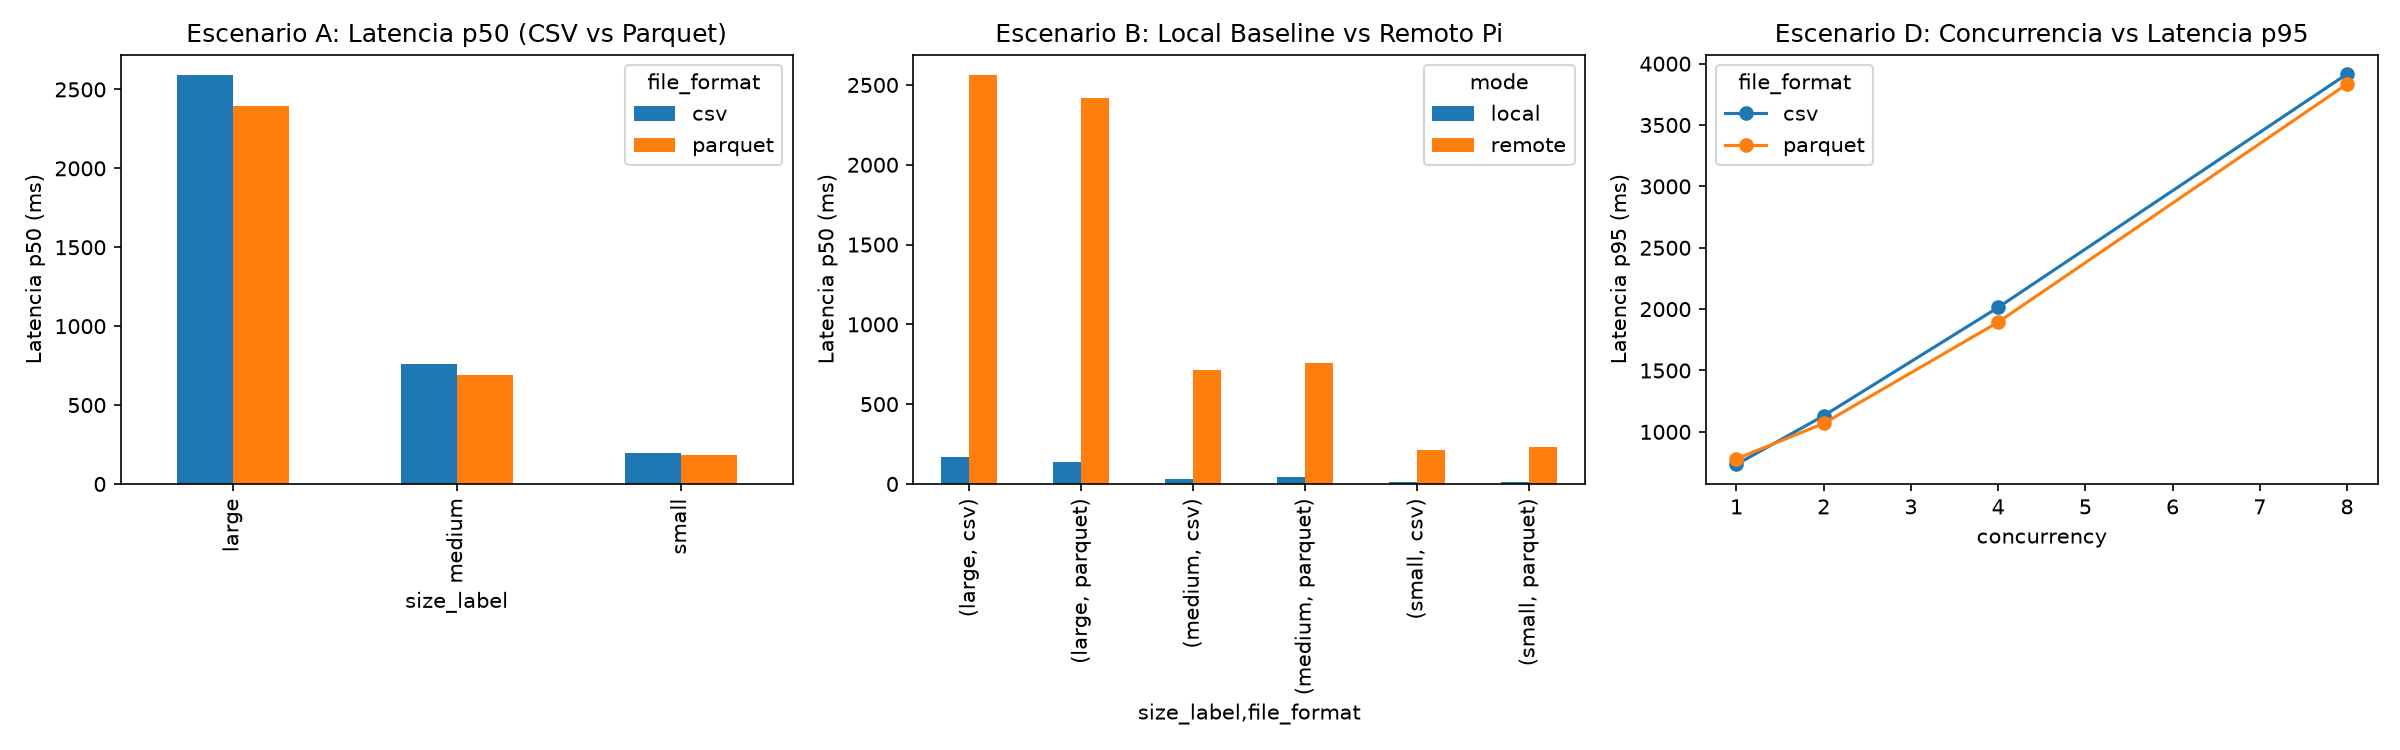
\includegraphics[width=\textwidth]{results/evaluation_plots.png}
    \caption{Comparación gráfica generada automáticamente para los Escenarios A (CSV vs. Parquet), B (Local vs. Remoto) y D (Escalabilidad bajo Concurrencia).}
    \label{fig:plots}
\end{figure}

\section{Conclusiones Basadas en Evidencia}
\begin{enumerate}
    \item \textbf{Elección de formato de almacenamiento}: \textbf{Parquet} es ampliamente superior para escritura intensiva ($12.6\times$ más rápido en disco), almacenamiento en nodos con tarjeta microSD limitada (hasta $7.66\times$ menor tamaño en disco) y consultas analíticas por columnas ($6.7\times$ menor tiempo de disco). \textbf{CSV} solo resulta competitivo en lecturas parciales de unas pocas filas contiguas al inicio del archivo (\texttt{read\_range}).
    \item \textbf{Identificación de cuellos de botella}: La instrumentación separada demostró que en lecturas remotas de datasets completos, el almacenamiento local en disco representa menos del 5\% del tiempo total, siendo la serialización y el transporte de red los factores dominantes.
    \item \textbf{Elección de protocolo de transporte}: \textbf{gRPC} reduce la latencia en peticiones pequeñas y medianas gracias a la gestión eficiente de canales HTTP/2, mientras que los \textbf{Sockets TCP con framing binario de 4 bytes} igualan o superan ligeramente el \textit{throughput} en transferencias masivas con menor sobrecarga de CPU.
\end{enumerate}

\end{document}
